\PassOptionsToPackage{unicode=true}{hyperref} % options for packages loaded elsewhere
\PassOptionsToPackage{hyphens}{url}
\PassOptionsToPackage{dvipsnames,svgnames*,x11names*}{xcolor}
%
\documentclass[]{article}
\usepackage{lmodern}
\usepackage{amssymb,amsmath}
\usepackage{ifxetex,ifluatex}
\usepackage{fixltx2e} % provides \textsubscript
\ifnum 0\ifxetex 1\fi\ifluatex 1\fi=0 % if pdftex
  \usepackage[T1]{fontenc}
  \usepackage[utf8]{inputenc}
  \usepackage{textcomp} % provides euro and other symbols
\else % if luatex or xelatex
  \usepackage{unicode-math}
  \defaultfontfeatures{Ligatures=TeX,Scale=MatchLowercase}
\fi
% use upquote if available, for straight quotes in verbatim environments
\IfFileExists{upquote.sty}{\usepackage{upquote}}{}
% use microtype if available
\IfFileExists{microtype.sty}{%
\usepackage[]{microtype}
\UseMicrotypeSet[protrusion]{basicmath} % disable protrusion for tt fonts
}{}
\IfFileExists{parskip.sty}{%
\usepackage{parskip}
}{% else
\setlength{\parindent}{0pt}
\setlength{\parskip}{6pt plus 2pt minus 1pt}
}
\usepackage{xcolor}
\usepackage{hyperref}
\hypersetup{
            pdftitle={Module 10: Recommended Exercises - Solutions},
            pdfauthor={Thiago G. Martins, Martina Hall, Stefanie Muff, Department of Mathematical Sciences, NTNU},
            colorlinks=true,
            linkcolor=Maroon,
            filecolor=Maroon,
            citecolor=Blue,
            urlcolor=blue,
            breaklinks=true}
\urlstyle{same}  % don't use monospace font for urls
\usepackage[margin=1in]{geometry}
\usepackage{color}
\usepackage{fancyvrb}
\newcommand{\VerbBar}{|}
\newcommand{\VERB}{\Verb[commandchars=\\\{\}]}
\DefineVerbatimEnvironment{Highlighting}{Verbatim}{commandchars=\\\{\}}
% Add ',fontsize=\small' for more characters per line
\usepackage{framed}
\definecolor{shadecolor}{RGB}{248,248,248}
\newenvironment{Shaded}{\begin{snugshade}}{\end{snugshade}}
\newcommand{\AlertTok}[1]{\textcolor[rgb]{0.94,0.16,0.16}{#1}}
\newcommand{\AnnotationTok}[1]{\textcolor[rgb]{0.56,0.35,0.01}{\textbf{\textit{#1}}}}
\newcommand{\AttributeTok}[1]{\textcolor[rgb]{0.77,0.63,0.00}{#1}}
\newcommand{\BaseNTok}[1]{\textcolor[rgb]{0.00,0.00,0.81}{#1}}
\newcommand{\BuiltInTok}[1]{#1}
\newcommand{\CharTok}[1]{\textcolor[rgb]{0.31,0.60,0.02}{#1}}
\newcommand{\CommentTok}[1]{\textcolor[rgb]{0.56,0.35,0.01}{\textit{#1}}}
\newcommand{\CommentVarTok}[1]{\textcolor[rgb]{0.56,0.35,0.01}{\textbf{\textit{#1}}}}
\newcommand{\ConstantTok}[1]{\textcolor[rgb]{0.00,0.00,0.00}{#1}}
\newcommand{\ControlFlowTok}[1]{\textcolor[rgb]{0.13,0.29,0.53}{\textbf{#1}}}
\newcommand{\DataTypeTok}[1]{\textcolor[rgb]{0.13,0.29,0.53}{#1}}
\newcommand{\DecValTok}[1]{\textcolor[rgb]{0.00,0.00,0.81}{#1}}
\newcommand{\DocumentationTok}[1]{\textcolor[rgb]{0.56,0.35,0.01}{\textbf{\textit{#1}}}}
\newcommand{\ErrorTok}[1]{\textcolor[rgb]{0.64,0.00,0.00}{\textbf{#1}}}
\newcommand{\ExtensionTok}[1]{#1}
\newcommand{\FloatTok}[1]{\textcolor[rgb]{0.00,0.00,0.81}{#1}}
\newcommand{\FunctionTok}[1]{\textcolor[rgb]{0.00,0.00,0.00}{#1}}
\newcommand{\ImportTok}[1]{#1}
\newcommand{\InformationTok}[1]{\textcolor[rgb]{0.56,0.35,0.01}{\textbf{\textit{#1}}}}
\newcommand{\KeywordTok}[1]{\textcolor[rgb]{0.13,0.29,0.53}{\textbf{#1}}}
\newcommand{\NormalTok}[1]{#1}
\newcommand{\OperatorTok}[1]{\textcolor[rgb]{0.81,0.36,0.00}{\textbf{#1}}}
\newcommand{\OtherTok}[1]{\textcolor[rgb]{0.56,0.35,0.01}{#1}}
\newcommand{\PreprocessorTok}[1]{\textcolor[rgb]{0.56,0.35,0.01}{\textit{#1}}}
\newcommand{\RegionMarkerTok}[1]{#1}
\newcommand{\SpecialCharTok}[1]{\textcolor[rgb]{0.00,0.00,0.00}{#1}}
\newcommand{\SpecialStringTok}[1]{\textcolor[rgb]{0.31,0.60,0.02}{#1}}
\newcommand{\StringTok}[1]{\textcolor[rgb]{0.31,0.60,0.02}{#1}}
\newcommand{\VariableTok}[1]{\textcolor[rgb]{0.00,0.00,0.00}{#1}}
\newcommand{\VerbatimStringTok}[1]{\textcolor[rgb]{0.31,0.60,0.02}{#1}}
\newcommand{\WarningTok}[1]{\textcolor[rgb]{0.56,0.35,0.01}{\textbf{\textit{#1}}}}
\usepackage{graphicx,grffile}
\makeatletter
\def\maxwidth{\ifdim\Gin@nat@width>\linewidth\linewidth\else\Gin@nat@width\fi}
\def\maxheight{\ifdim\Gin@nat@height>\textheight\textheight\else\Gin@nat@height\fi}
\makeatother
% Scale images if necessary, so that they will not overflow the page
% margins by default, and it is still possible to overwrite the defaults
% using explicit options in \includegraphics[width, height, ...]{}
\setkeys{Gin}{width=\maxwidth,height=\maxheight,keepaspectratio}
\setlength{\emergencystretch}{3em}  % prevent overfull lines
\providecommand{\tightlist}{%
  \setlength{\itemsep}{0pt}\setlength{\parskip}{0pt}}
\setcounter{secnumdepth}{0}
% Redefines (sub)paragraphs to behave more like sections
\ifx\paragraph\undefined\else
\let\oldparagraph\paragraph
\renewcommand{\paragraph}[1]{\oldparagraph{#1}\mbox{}}
\fi
\ifx\subparagraph\undefined\else
\let\oldsubparagraph\subparagraph
\renewcommand{\subparagraph}[1]{\oldsubparagraph{#1}\mbox{}}
\fi

% set default figure placement to htbp
\makeatletter
\def\fps@figure{htbp}
\makeatother

\usepackage{etoolbox}
\makeatletter
\providecommand{\subtitle}[1]{% add subtitle to \maketitle
  \apptocmd{\@title}{\par {\large #1 \par}}{}{}
}
\makeatother

\title{Module 10: Recommended Exercises - Solutions}
\providecommand{\subtitle}[1]{}
\subtitle{TMA4268 Statistical Learning V2020}
\author{Thiago G. Martins, Martina Hall, Stefanie Muff, Department of
Mathematical Sciences, NTNU}
\date{March 14, 2020}

\begin{document}
\maketitle

\hypertarget{recommended-exercise-1}{%
\section{Recommended exercise 1}\label{recommended-exercise-1}}

Get the data by loading it

\begin{Shaded}
\begin{Highlighting}[]
\KeywordTok{load}\NormalTok{(}\StringTok{"pca-examples.rdata"}\NormalTok{)}

\CommentTok{# We will work with nyt.frame}
\NormalTok{nyt_data =}\StringTok{ }\NormalTok{nyt.frame}
\end{Highlighting}
\end{Shaded}

Compute the PCA

\begin{Shaded}
\begin{Highlighting}[]
\NormalTok{nyt_pca =}\StringTok{ }\KeywordTok{prcomp}\NormalTok{(nyt_data[, }\DecValTok{-1}\NormalTok{])}
\end{Highlighting}
\end{Shaded}

\hypertarget{default-biplot}{%
\subsection{Default biplot}\label{default-biplot}}

Too much information on the graph, we should select only a few loading
vectors to display.

\begin{Shaded}
\begin{Highlighting}[]
\KeywordTok{biplot}\NormalTok{(nyt_pca, }\DataTypeTok{scale =} \DecValTok{0}\NormalTok{)}
\end{Highlighting}
\end{Shaded}

\begin{center}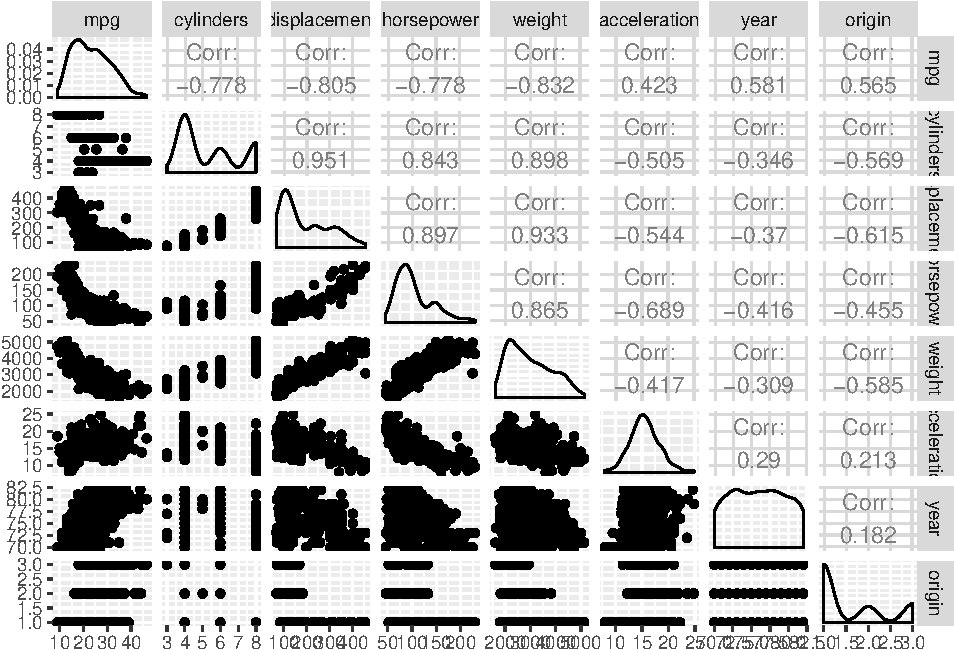
\includegraphics{RecEx10-sol_files/figure-latex/unnamed-chunk-3-1} \end{center}

Lets pick some words with high PC1 weight and some words with high PC2
weight. Only looking at the graph we can see that PC1 is associated with
music and PC2 with art.

\begin{Shaded}
\begin{Highlighting}[]
\NormalTok{nyt_loading =}\StringTok{ }\NormalTok{nyt_pca}\OperatorTok{$}\NormalTok{rotation[, }\DecValTok{1}\OperatorTok{:}\DecValTok{2}\NormalTok{]}
\NormalTok{informative_loadings =}\StringTok{ }\KeywordTok{rbind}\NormalTok{(}\KeywordTok{head}\NormalTok{(nyt_loading[}\KeywordTok{order}\NormalTok{(nyt_loading[, }\DecValTok{1}\NormalTok{], }\DataTypeTok{decreasing =} \OtherTok{TRUE}\NormalTok{), }
\NormalTok{    ]), }\KeywordTok{head}\NormalTok{(nyt_loading[}\KeywordTok{order}\NormalTok{(nyt_loading[, }\DecValTok{2}\NormalTok{], }\DataTypeTok{decreasing =} \OtherTok{TRUE}\NormalTok{), ]))}

\KeywordTok{biplot}\NormalTok{(}\DataTypeTok{x =}\NormalTok{ nyt_pca}\OperatorTok{$}\NormalTok{x[, }\DecValTok{1}\OperatorTok{:}\DecValTok{2}\NormalTok{], }\DataTypeTok{y =}\NormalTok{ informative_loadings, }\DataTypeTok{scale =} \DecValTok{0}\NormalTok{)}
\end{Highlighting}
\end{Shaded}

\begin{center}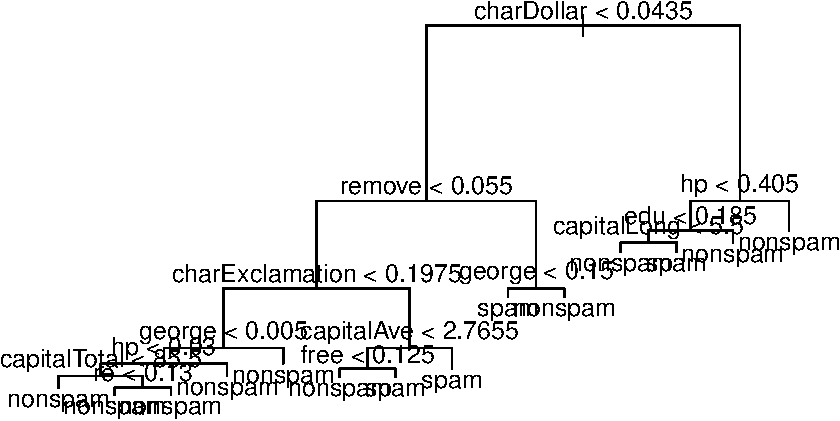
\includegraphics{RecEx10-sol_files/figure-latex/unnamed-chunk-4-1} \end{center}

\hypertarget{proportion-of-variance-explained-pve}{%
\subsection{Proportion of variance explained
(PVE)}\label{proportion-of-variance-explained-pve}}

The numbers below show that although the graphs based on PC1 and PC2
give some insight about document types, the first two PCs explain only
small portion of the variability contained in the data.

\begin{Shaded}
\begin{Highlighting}[]
\NormalTok{pr.var =}\StringTok{ }\NormalTok{nyt_pca}\OperatorTok{$}\NormalTok{sdev}\OperatorTok{^}\DecValTok{2}
\NormalTok{pr.var}
\end{Highlighting}
\end{Shaded}

\begin{verbatim}
##   [1] 1.988751e-02 1.862759e-02 1.724294e-02 1.537218e-02 1.440484e-02
##   [6] 1.393311e-02 1.313569e-02 1.285084e-02 1.228344e-02 1.207883e-02
##  [11] 1.191209e-02 1.178849e-02 1.169569e-02 1.159828e-02 1.140559e-02
##  [16] 1.133632e-02 1.124601e-02 1.113017e-02 1.110012e-02 1.095067e-02
##  [21] 1.086651e-02 1.072844e-02 1.060126e-02 1.058186e-02 1.056528e-02
##  [26] 1.045440e-02 1.035742e-02 1.032494e-02 1.030728e-02 1.022799e-02
##  [31] 1.010669e-02 1.004629e-02 1.001430e-02 9.977470e-03 9.945853e-03
##  [36] 9.885270e-03 9.732177e-03 9.679161e-03 9.636696e-03 9.578010e-03
##  [41] 9.535481e-03 9.466407e-03 9.437146e-03 9.399834e-03 9.307165e-03
##  [46] 9.203604e-03 9.179709e-03 9.133426e-03 9.102611e-03 9.041575e-03
##  [51] 8.998882e-03 8.925813e-03 8.884005e-03 8.848814e-03 8.799356e-03
##  [56] 8.747191e-03 8.717555e-03 8.643816e-03 8.559859e-03 8.529536e-03
##  [61] 8.469763e-03 8.467367e-03 8.393981e-03 8.376228e-03 8.251717e-03
##  [66] 8.235627e-03 8.149720e-03 8.123239e-03 8.044627e-03 8.015822e-03
##  [71] 7.982089e-03 7.888293e-03 7.810759e-03 7.795754e-03 7.774335e-03
##  [76] 7.683500e-03 7.631978e-03 7.615316e-03 7.548048e-03 7.482993e-03
##  [81] 7.419521e-03 7.366235e-03 7.340519e-03 7.288173e-03 7.269157e-03
##  [86] 7.175837e-03 7.160695e-03 7.109025e-03 7.036169e-03 6.984169e-03
##  [91] 6.892596e-03 6.805417e-03 6.670563e-03 6.566518e-03 6.466879e-03
##  [96] 6.420743e-03 6.337557e-03 6.233789e-03 6.191162e-03 6.025576e-03
## [101] 5.283112e-03 3.582418e-32
\end{verbatim}

We can then compute the proportion of variance explained by each
principal component

\begin{Shaded}
\begin{Highlighting}[]
\NormalTok{pve =}\StringTok{ }\NormalTok{pr.var}\OperatorTok{/}\KeywordTok{sum}\NormalTok{(pr.var)}
\NormalTok{pve}
\end{Highlighting}
\end{Shaded}

\begin{verbatim}
##   [1] 2.093766e-02 1.961121e-02 1.815344e-02 1.618390e-02 1.516547e-02
##   [6] 1.466884e-02 1.382931e-02 1.352942e-02 1.293206e-02 1.271664e-02
##  [11] 1.254110e-02 1.241097e-02 1.231328e-02 1.221072e-02 1.200786e-02
##  [16] 1.193492e-02 1.183985e-02 1.171789e-02 1.168626e-02 1.152892e-02
##  [21] 1.144031e-02 1.129495e-02 1.116105e-02 1.114063e-02 1.112318e-02
##  [26] 1.100644e-02 1.090434e-02 1.087014e-02 1.085155e-02 1.076808e-02
##  [31] 1.064037e-02 1.057678e-02 1.054310e-02 1.050432e-02 1.047104e-02
##  [36] 1.040726e-02 1.024608e-02 1.019026e-02 1.014556e-02 1.008377e-02
##  [41] 1.003900e-02 9.966275e-03 9.935469e-03 9.896187e-03 9.798624e-03
##  [46] 9.689594e-03 9.664439e-03 9.615711e-03 9.583269e-03 9.519011e-03
##  [51] 9.474062e-03 9.397135e-03 9.353120e-03 9.316071e-03 9.264001e-03
##  [56] 9.209081e-03 9.177880e-03 9.100248e-03 9.011858e-03 8.979933e-03
##  [61] 8.917003e-03 8.914481e-03 8.837220e-03 8.818530e-03 8.687444e-03
##  [66] 8.670504e-03 8.580061e-03 8.552182e-03 8.469419e-03 8.439092e-03
##  [71] 8.403578e-03 8.304829e-03 8.223201e-03 8.207404e-03 8.184854e-03
##  [76] 8.089223e-03 8.034980e-03 8.017438e-03 7.946618e-03 7.878128e-03
##  [81] 7.811304e-03 7.755204e-03 7.728131e-03 7.673021e-03 7.653000e-03
##  [86] 7.554753e-03 7.538811e-03 7.484412e-03 7.407710e-03 7.352964e-03
##  [91] 7.256556e-03 7.164773e-03 7.022798e-03 6.913259e-03 6.808359e-03
##  [96] 6.759786e-03 6.672208e-03 6.562961e-03 6.518083e-03 6.343753e-03
## [101] 5.562084e-03 3.771586e-32
\end{verbatim}

We can plot the PVE explained by each component, as well as the
cumulative PVE, as follows:

\begin{Shaded}
\begin{Highlighting}[]
\KeywordTok{plot}\NormalTok{(pve, }\DataTypeTok{xlab =} \StringTok{"Principal Component"}\NormalTok{, }\DataTypeTok{ylab =} \StringTok{"Proportion of Variance Explained"}\NormalTok{, }
    \DataTypeTok{ylim =} \KeywordTok{c}\NormalTok{(}\DecValTok{0}\NormalTok{, }\DecValTok{1}\NormalTok{), }\DataTypeTok{type =} \StringTok{"b"}\NormalTok{)}
\end{Highlighting}
\end{Shaded}

\begin{center}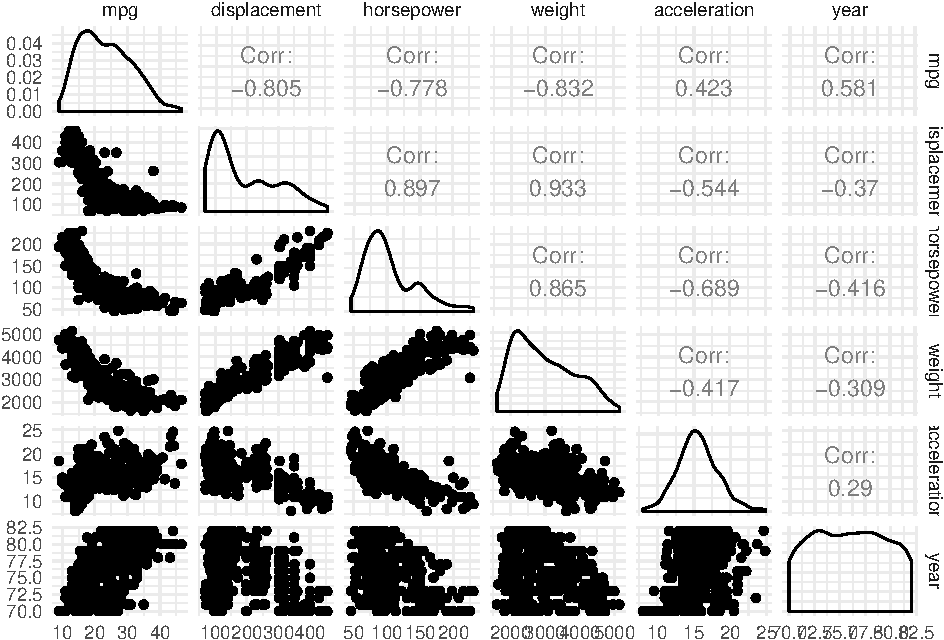
\includegraphics{RecEx10-sol_files/figure-latex/unnamed-chunk-7-1} \end{center}

\begin{Shaded}
\begin{Highlighting}[]
\KeywordTok{plot}\NormalTok{(}\KeywordTok{cumsum}\NormalTok{(pve), }\DataTypeTok{xlab =} \StringTok{"Principal Component"}\NormalTok{, }\DataTypeTok{ylab =} \StringTok{"Cumulative Proportion of Variance Explained"}\NormalTok{, }
    \DataTypeTok{ylim =} \KeywordTok{c}\NormalTok{(}\DecValTok{0}\NormalTok{, }\DecValTok{1}\NormalTok{), }\DataTypeTok{type =} \StringTok{"b"}\NormalTok{)}
\end{Highlighting}
\end{Shaded}

\begin{center}\includegraphics{RecEx10-sol_files/figure-latex/unnamed-chunk-7-2} \end{center}

\hypertarget{recommended-exercise-2}{%
\section{Recommended exercise 2}\label{recommended-exercise-2}}

The answer is on page 388 of the book, with the explanation around
Equation (10.12).

\hypertarget{recommended-exercise-3}{%
\section{Recommended exercise 3}\label{recommended-exercise-3}}

\(k\)-means clustering:

\begin{Shaded}
\begin{Highlighting}[]
\NormalTok{km.out =}\StringTok{ }\KeywordTok{kmeans}\NormalTok{(nyt_data[, }\DecValTok{-1}\NormalTok{], }\DecValTok{2}\NormalTok{, }\DataTypeTok{nstart =} \DecValTok{20}\NormalTok{)}
\end{Highlighting}
\end{Shaded}

\hypertarget{cluster-assignments}{%
\subsection{Cluster assignments}\label{cluster-assignments}}

\begin{Shaded}
\begin{Highlighting}[]
\NormalTok{km.out}\OperatorTok{$}\NormalTok{cluster}
\end{Highlighting}
\end{Shaded}

\begin{verbatim}
##   [1] 2 2 2 2 2 2 2 2 2 2 2 2 2 2 2 2 2 2 1 2 2 2 2 1 2 2 2 2 2 2 2 2 2 1 1
##  [36] 1 2 2 1 2 2 2 2 2 2 2 2 2 2 2 2 1 2 2 2 2 1 1 1 1 1 1 2 1 1 1 1 1 1 1
##  [71] 1 1 1 2 1 1 1 1 1 1 1 1 1 1 1 1 1 2 1 1 1 1 1 1 1 2 1 1 1 1 1 1
\end{verbatim}

\hypertarget{plot-the-data}{%
\subsection{Plot the data}\label{plot-the-data}}

To plot the data we need to use the PCA projections. Below we will use
the plot based on PCA with true labels (A for art and M for music) and
compare with the plot that color the points according to the \(k\)-means
clustering.

\begin{Shaded}
\begin{Highlighting}[]
\CommentTok{# PCA with true labels}
\KeywordTok{plot}\NormalTok{(nyt_pca}\OperatorTok{$}\NormalTok{x[, }\DecValTok{1}\OperatorTok{:}\DecValTok{2}\NormalTok{], }\DataTypeTok{type =} \StringTok{"n"}\NormalTok{)}
\KeywordTok{points}\NormalTok{(nyt_pca}\OperatorTok{$}\NormalTok{x[nyt_data[, }\StringTok{"class.labels"}\NormalTok{] }\OperatorTok{==}\StringTok{ "art"}\NormalTok{, }\DecValTok{1}\OperatorTok{:}\DecValTok{2}\NormalTok{], }\DataTypeTok{pch =} \StringTok{"A"}\NormalTok{)}
\KeywordTok{points}\NormalTok{(nyt_pca}\OperatorTok{$}\NormalTok{x[nyt_data[, }\StringTok{"class.labels"}\NormalTok{] }\OperatorTok{==}\StringTok{ "music"}\NormalTok{, }\DecValTok{1}\OperatorTok{:}\DecValTok{2}\NormalTok{], }\DataTypeTok{pch =} \StringTok{"M"}\NormalTok{)}
\end{Highlighting}
\end{Shaded}

\begin{center}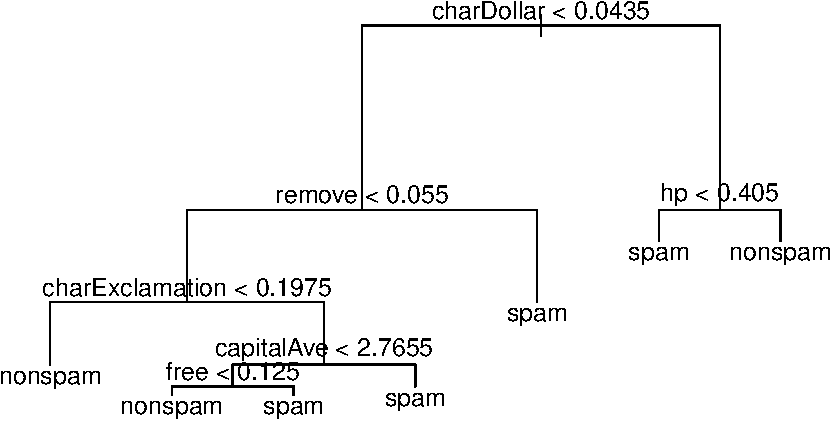
\includegraphics{RecEx10-sol_files/figure-latex/unnamed-chunk-10-1} \end{center}

PCA with true labels but colored by \(k\)-means clustering

\begin{Shaded}
\begin{Highlighting}[]
\KeywordTok{plot}\NormalTok{(nyt_pca}\OperatorTok{$}\NormalTok{x[, }\DecValTok{1}\OperatorTok{:}\DecValTok{2}\NormalTok{], }\DataTypeTok{type =} \StringTok{"n"}\NormalTok{)}
\KeywordTok{points}\NormalTok{(nyt_pca}\OperatorTok{$}\NormalTok{x[nyt_data[, }\StringTok{"class.labels"}\NormalTok{] }\OperatorTok{==}\StringTok{ "art"}\NormalTok{, }\DecValTok{1}\OperatorTok{:}\DecValTok{2}\NormalTok{], }\DataTypeTok{pch =} \StringTok{"A"}\NormalTok{, }\DataTypeTok{col =}\NormalTok{ (km.out}\OperatorTok{$}\NormalTok{cluster }\OperatorTok{+}\StringTok{ }
\StringTok{    }\DecValTok{1}\NormalTok{)[nyt_data[, }\StringTok{"class.labels"}\NormalTok{] }\OperatorTok{==}\StringTok{ "art"}\NormalTok{])}
\KeywordTok{points}\NormalTok{(nyt_pca}\OperatorTok{$}\NormalTok{x[nyt_data[, }\StringTok{"class.labels"}\NormalTok{] }\OperatorTok{==}\StringTok{ "music"}\NormalTok{, }\DecValTok{1}\OperatorTok{:}\DecValTok{2}\NormalTok{], }\DataTypeTok{pch =} \StringTok{"M"}\NormalTok{, }\DataTypeTok{col =}\NormalTok{ (km.out}\OperatorTok{$}\NormalTok{cluster }\OperatorTok{+}\StringTok{ }
\StringTok{    }\DecValTok{1}\NormalTok{)[nyt_data[, }\StringTok{"class.labels"}\NormalTok{] }\OperatorTok{==}\StringTok{ "music"}\NormalTok{])}
\end{Highlighting}
\end{Shaded}

\begin{center}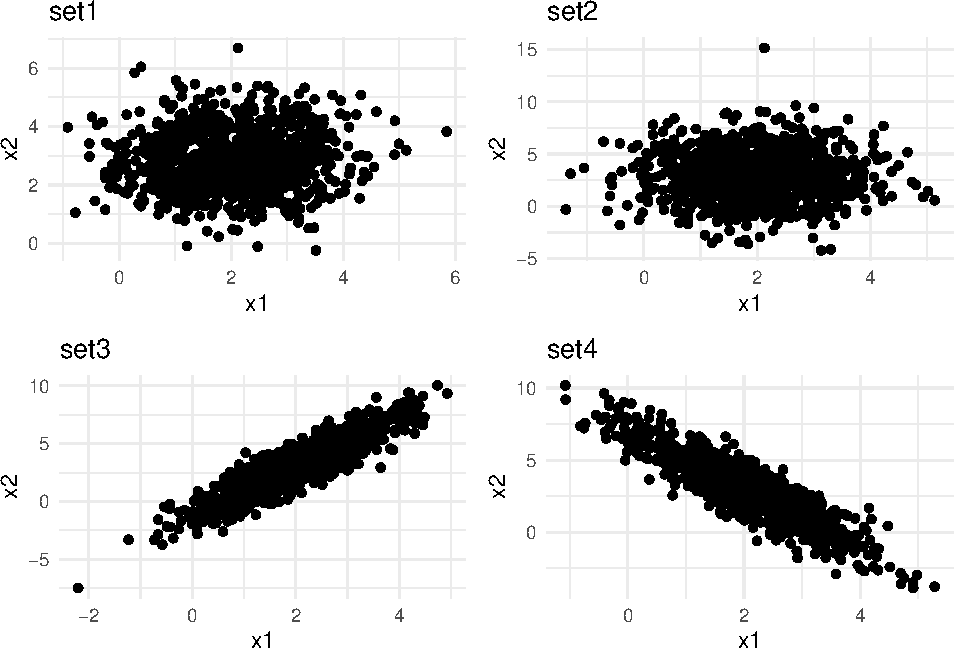
\includegraphics{RecEx10-sol_files/figure-latex/unnamed-chunk-11-1} \end{center}

\hypertarget{recommended-exercise-4}{%
\section{Recommended exercise 4}\label{recommended-exercise-4}}

\hypertarget{perform-hierarchical-clustering}{%
\subsection{Perform hierarchical
clustering}\label{perform-hierarchical-clustering}}

I will use euclidean distance and complete linkage

\begin{Shaded}
\begin{Highlighting}[]
\NormalTok{hc.complete =}\StringTok{ }\KeywordTok{hclust}\NormalTok{(}\KeywordTok{dist}\NormalTok{(nyt_data[, }\DecValTok{-1}\NormalTok{]), }\DataTypeTok{method =} \StringTok{"complete"}\NormalTok{)}
\KeywordTok{str}\NormalTok{(hc.complete)}
\end{Highlighting}
\end{Shaded}

\begin{verbatim}
## List of 7
##  $ merge      : int [1:101, 1:2] -46 -84 -68 -18 -65 -23 -71 -64 -95 -37 ...
##  $ height     : num [1:101] 1.1 1.22 1.22 1.23 1.24 ...
##  $ order      : int [1:102] 94 24 93 16 46 55 59 87 39 90 ...
##  $ labels     : NULL
##  $ method     : chr "complete"
##  $ call       : language hclust(d = dist(nyt_data[, -1]), method = "complete")
##  $ dist.method: chr "euclidean"
##  - attr(*, "class")= chr "hclust"
\end{verbatim}

\hypertarget{plot-dendograms}{%
\subsection{Plot dendograms}\label{plot-dendograms}}

\begin{Shaded}
\begin{Highlighting}[]
\KeywordTok{plot}\NormalTok{(hc.complete, }\DataTypeTok{main =} \StringTok{"Complete Linkage"}\NormalTok{, }\DataTypeTok{labels =} \KeywordTok{as.character}\NormalTok{(nyt_data[, }
    \DecValTok{1}\NormalTok{]), }\DataTypeTok{xlab =} \StringTok{""}\NormalTok{, }\DataTypeTok{sub =} \StringTok{""}\NormalTok{, }\DataTypeTok{cex =} \FloatTok{0.9}\NormalTok{)}
\end{Highlighting}
\end{Shaded}

\begin{center}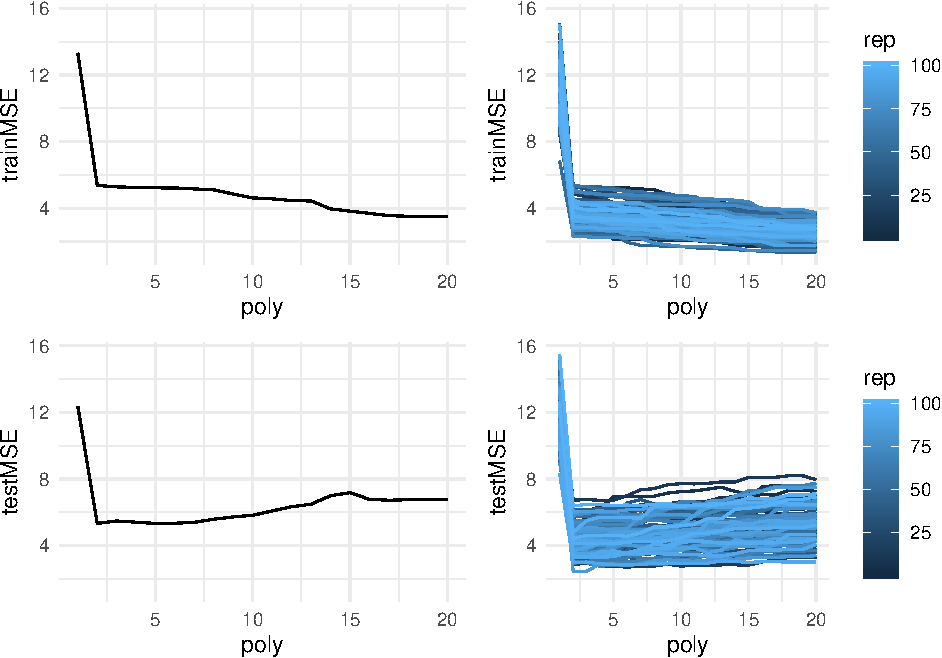
\includegraphics{RecEx10-sol_files/figure-latex/unnamed-chunk-13-1} \end{center}

\hypertarget{cluster-assignment}{%
\subsection{Cluster assignment}\label{cluster-assignment}}

\begin{Shaded}
\begin{Highlighting}[]
\NormalTok{hc.clusters =}\StringTok{ }\KeywordTok{cutree}\NormalTok{(hc.complete, }\DecValTok{2}\NormalTok{)}
\end{Highlighting}
\end{Shaded}

\hypertarget{plot-the-data-1}{%
\subsection{Plot the data}\label{plot-the-data-1}}

Based on the cluster assignment above and the plots below we see that
hierarchical clustering performs worse than \(k\)-means for the same
number of clusters (K=2)

\begin{Shaded}
\begin{Highlighting}[]
\CommentTok{# PCA with true labels}
\KeywordTok{plot}\NormalTok{(nyt_pca}\OperatorTok{$}\NormalTok{x[, }\DecValTok{1}\OperatorTok{:}\DecValTok{2}\NormalTok{], }\DataTypeTok{type =} \StringTok{"n"}\NormalTok{)}
\KeywordTok{points}\NormalTok{(nyt_pca}\OperatorTok{$}\NormalTok{x[nyt_data[, }\StringTok{"class.labels"}\NormalTok{] }\OperatorTok{==}\StringTok{ "art"}\NormalTok{, }\DecValTok{1}\OperatorTok{:}\DecValTok{2}\NormalTok{], }\DataTypeTok{pch =} \StringTok{"A"}\NormalTok{)}
\KeywordTok{points}\NormalTok{(nyt_pca}\OperatorTok{$}\NormalTok{x[nyt_data[, }\StringTok{"class.labels"}\NormalTok{] }\OperatorTok{==}\StringTok{ "music"}\NormalTok{, }\DecValTok{1}\OperatorTok{:}\DecValTok{2}\NormalTok{], }\DataTypeTok{pch =} \StringTok{"M"}\NormalTok{)}
\end{Highlighting}
\end{Shaded}

\begin{center}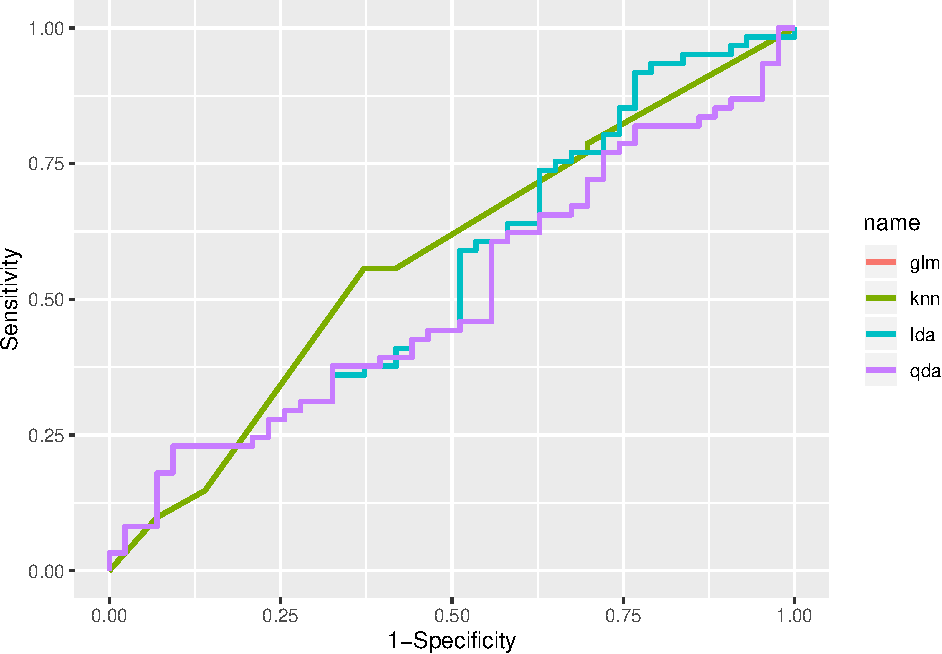
\includegraphics{RecEx10-sol_files/figure-latex/unnamed-chunk-15-1} \end{center}

PCA with true labels but colored by \(k\)-means clustering

\begin{Shaded}
\begin{Highlighting}[]
\KeywordTok{plot}\NormalTok{(nyt_pca}\OperatorTok{$}\NormalTok{x[, }\DecValTok{1}\OperatorTok{:}\DecValTok{2}\NormalTok{], }\DataTypeTok{type =} \StringTok{"n"}\NormalTok{)}
\KeywordTok{points}\NormalTok{(nyt_pca}\OperatorTok{$}\NormalTok{x[nyt_data[, }\StringTok{"class.labels"}\NormalTok{] }\OperatorTok{==}\StringTok{ "art"}\NormalTok{, }\DecValTok{1}\OperatorTok{:}\DecValTok{2}\NormalTok{], }\DataTypeTok{pch =} \StringTok{"A"}\NormalTok{, }\DataTypeTok{col =}\NormalTok{ (hc.clusters }\OperatorTok{+}\StringTok{ }
\StringTok{    }\DecValTok{1}\NormalTok{)[nyt_data[, }\StringTok{"class.labels"}\NormalTok{] }\OperatorTok{==}\StringTok{ "art"}\NormalTok{])}
\KeywordTok{points}\NormalTok{(nyt_pca}\OperatorTok{$}\NormalTok{x[nyt_data[, }\StringTok{"class.labels"}\NormalTok{] }\OperatorTok{==}\StringTok{ "music"}\NormalTok{, }\DecValTok{1}\OperatorTok{:}\DecValTok{2}\NormalTok{], }\DataTypeTok{pch =} \StringTok{"M"}\NormalTok{, }\DataTypeTok{col =}\NormalTok{ (hc.clusters }\OperatorTok{+}\StringTok{ }
\StringTok{    }\DecValTok{1}\NormalTok{)[nyt_data[, }\StringTok{"class.labels"}\NormalTok{] }\OperatorTok{==}\StringTok{ "music"}\NormalTok{])}
\end{Highlighting}
\end{Shaded}

\begin{center}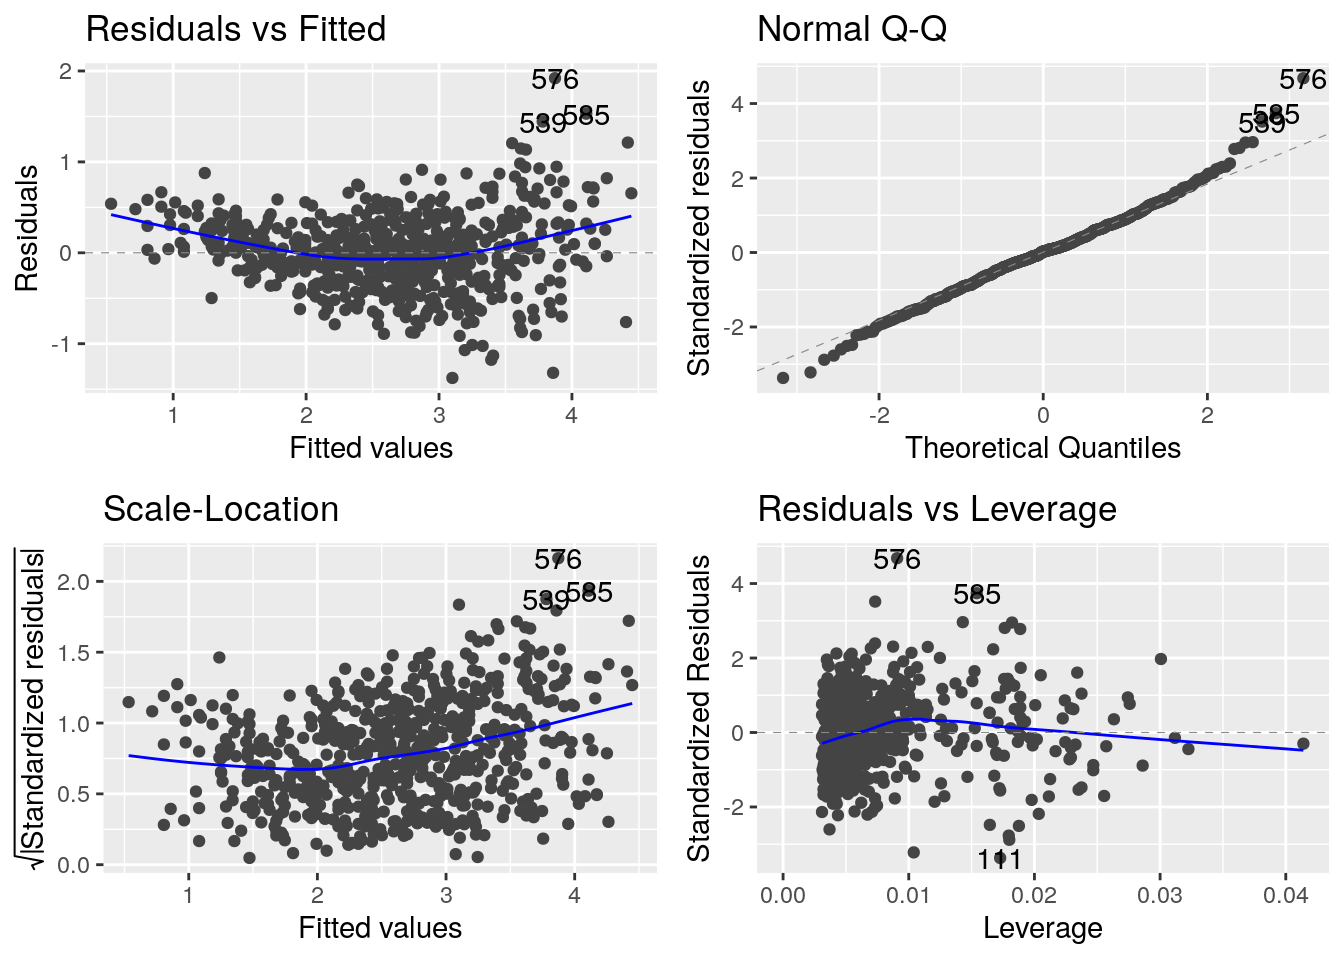
\includegraphics{RecEx10-sol_files/figure-latex/unnamed-chunk-16-1} \end{center}

Lets see if single linkage or average linkage performs better.

\begin{Shaded}
\begin{Highlighting}[]
\CommentTok{# hierachical clustering}
\NormalTok{hc.single =}\StringTok{ }\KeywordTok{hclust}\NormalTok{(}\KeywordTok{dist}\NormalTok{(nyt_data[, }\DecValTok{-1}\NormalTok{]), }\DataTypeTok{method =} \StringTok{"single"}\NormalTok{)}
\NormalTok{hc.average =}\StringTok{ }\KeywordTok{hclust}\NormalTok{(}\KeywordTok{dist}\NormalTok{(nyt_data[, }\DecValTok{-1}\NormalTok{]), }\DataTypeTok{method =} \StringTok{"average"}\NormalTok{)}
\end{Highlighting}
\end{Shaded}

\#plot dendogram

\begin{Shaded}
\begin{Highlighting}[]
\KeywordTok{par}\NormalTok{(}\DataTypeTok{mfrow =} \KeywordTok{c}\NormalTok{(}\DecValTok{1}\NormalTok{, }\DecValTok{2}\NormalTok{))}
\KeywordTok{plot}\NormalTok{(hc.single, }\DataTypeTok{main =} \StringTok{"Single Linkage"}\NormalTok{, }\DataTypeTok{labels =} \KeywordTok{as.character}\NormalTok{(nyt_data[, }\DecValTok{1}\NormalTok{]), }
    \DataTypeTok{xlab =} \StringTok{""}\NormalTok{, }\DataTypeTok{sub =} \StringTok{""}\NormalTok{, }\DataTypeTok{cex =} \FloatTok{0.9}\NormalTok{)}
\KeywordTok{plot}\NormalTok{(hc.average, }\DataTypeTok{main =} \StringTok{"Average Linkage"}\NormalTok{, }\DataTypeTok{labels =} \KeywordTok{as.character}\NormalTok{(nyt_data[, }
    \DecValTok{1}\NormalTok{]), }\DataTypeTok{xlab =} \StringTok{""}\NormalTok{, }\DataTypeTok{sub =} \StringTok{""}\NormalTok{, }\DataTypeTok{cex =} \FloatTok{0.9}\NormalTok{)}
\end{Highlighting}
\end{Shaded}

\begin{center}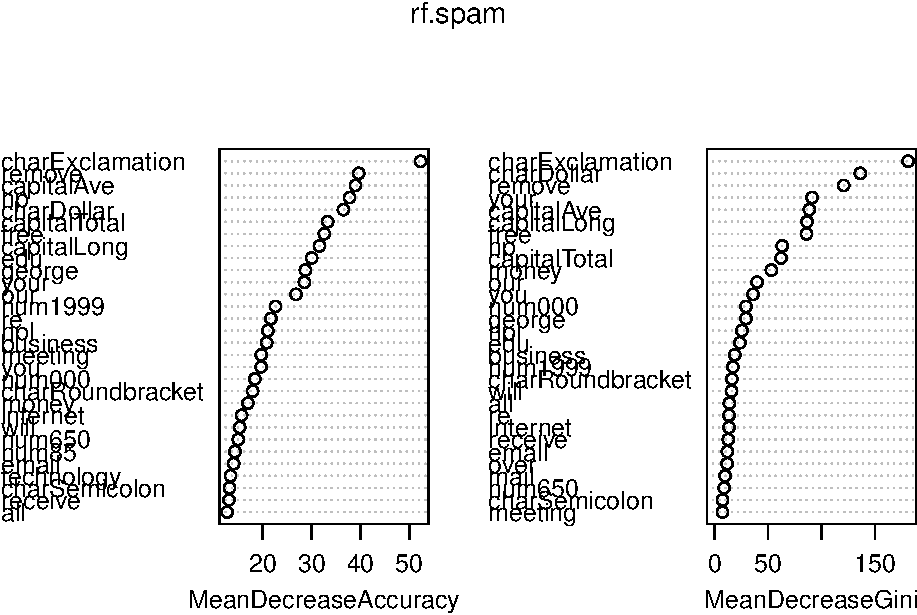
\includegraphics{RecEx10-sol_files/figure-latex/unnamed-chunk-18-1} \end{center}

\begin{Shaded}
\begin{Highlighting}[]
\CommentTok{# divide into clusters}
\NormalTok{hc.clustersSingle =}\StringTok{ }\KeywordTok{cutree}\NormalTok{(hc.single, }\DecValTok{2}\NormalTok{)}
\NormalTok{hc.clustersAverage =}\StringTok{ }\KeywordTok{cutree}\NormalTok{(hc.average, }\DecValTok{2}\NormalTok{)}
\end{Highlighting}
\end{Shaded}

Plot clusters in PC1 and PC2-dimension

\begin{Shaded}
\begin{Highlighting}[]
\KeywordTok{par}\NormalTok{(}\DataTypeTok{mfrow =} \KeywordTok{c}\NormalTok{(}\DecValTok{2}\NormalTok{, }\DecValTok{1}\NormalTok{))}
\KeywordTok{plot}\NormalTok{(nyt_pca}\OperatorTok{$}\NormalTok{x[, }\DecValTok{1}\OperatorTok{:}\DecValTok{2}\NormalTok{], }\DataTypeTok{type =} \StringTok{"n"}\NormalTok{)}
\KeywordTok{points}\NormalTok{(nyt_pca}\OperatorTok{$}\NormalTok{x[nyt_data[, }\StringTok{"class.labels"}\NormalTok{] }\OperatorTok{==}\StringTok{ "art"}\NormalTok{, }\DecValTok{1}\OperatorTok{:}\DecValTok{2}\NormalTok{], }\DataTypeTok{pch =} \StringTok{"A"}\NormalTok{, }\DataTypeTok{col =}\NormalTok{ (hc.clustersSingle }\OperatorTok{+}\StringTok{ }
\StringTok{    }\DecValTok{1}\NormalTok{)[nyt_data[, }\StringTok{"class.labels"}\NormalTok{] }\OperatorTok{==}\StringTok{ "art"}\NormalTok{])}
\KeywordTok{points}\NormalTok{(nyt_pca}\OperatorTok{$}\NormalTok{x[nyt_data[, }\StringTok{"class.labels"}\NormalTok{] }\OperatorTok{==}\StringTok{ "music"}\NormalTok{, }\DecValTok{1}\OperatorTok{:}\DecValTok{2}\NormalTok{], }\DataTypeTok{pch =} \StringTok{"M"}\NormalTok{, }\DataTypeTok{col =}\NormalTok{ (hc.clustersSingle }\OperatorTok{+}\StringTok{ }
\StringTok{    }\DecValTok{1}\NormalTok{)[nyt_data[, }\StringTok{"class.labels"}\NormalTok{] }\OperatorTok{==}\StringTok{ "music"}\NormalTok{])}
\KeywordTok{plot}\NormalTok{(nyt_pca}\OperatorTok{$}\NormalTok{x[, }\DecValTok{1}\OperatorTok{:}\DecValTok{2}\NormalTok{], }\DataTypeTok{type =} \StringTok{"n"}\NormalTok{)}
\KeywordTok{points}\NormalTok{(nyt_pca}\OperatorTok{$}\NormalTok{x[nyt_data[, }\StringTok{"class.labels"}\NormalTok{] }\OperatorTok{==}\StringTok{ "art"}\NormalTok{, }\DecValTok{1}\OperatorTok{:}\DecValTok{2}\NormalTok{], }\DataTypeTok{pch =} \StringTok{"A"}\NormalTok{, }\DataTypeTok{col =}\NormalTok{ (hc.clustersAverage }\OperatorTok{+}\StringTok{ }
\StringTok{    }\DecValTok{1}\NormalTok{)[nyt_data[, }\StringTok{"class.labels"}\NormalTok{] }\OperatorTok{==}\StringTok{ "art"}\NormalTok{])}
\KeywordTok{points}\NormalTok{(nyt_pca}\OperatorTok{$}\NormalTok{x[nyt_data[, }\StringTok{"class.labels"}\NormalTok{] }\OperatorTok{==}\StringTok{ "music"}\NormalTok{, }\DecValTok{1}\OperatorTok{:}\DecValTok{2}\NormalTok{], }\DataTypeTok{pch =} \StringTok{"M"}\NormalTok{, }\DataTypeTok{col =}\NormalTok{ (hc.clustersAverage }\OperatorTok{+}\StringTok{ }
\StringTok{    }\DecValTok{1}\NormalTok{)[nyt_data[, }\StringTok{"class.labels"}\NormalTok{] }\OperatorTok{==}\StringTok{ "music"}\NormalTok{])}
\end{Highlighting}
\end{Shaded}

\begin{center}\includegraphics{RecEx10-sol_files/figure-latex/unnamed-chunk-19-1} \end{center}

Doesn't seem to provide a better fit than complete.

\end{document}
